% This is a template document, a working progress, trying to replicate the UWindsor thesis template docx

% Table of Contents: All front matter is listed starting with Declaration
% Front matter assigned Roman numerals; chapters, pages numbered in Arabic numerals starting at one (1)
% Margins: 1 inch everywhere; 1 ½ inch on leftrecommended

\documentclass[12pt,letterpaper,oneside]{report}

% beginning of preambles

\usepackage{ifxetex} %  To make the document support both pdfLaTeX and Lua / XeLaTeX
\ifxetex
\usepackage{fontspec}
\defaultfontfeatures{Ligatures=TeX} % To support LaTeX quoting style
\usepackage{unicode-math} % for XITS
\setmainfont{XITS} % Any system font and font packages that are available as OpenType or TrueType
\setmathfont{XITS Math}
\else
\usepackage[utf8]{inputenc}
\usepackage[T1]{fontenc} % make sure cm-super is installed
\usepackage{lmodern} %\usefont{T1}{cmr}{m}{n} % for local font selection
\usepackage{textcomp} % \textdegree to print the degree sign for temperature and angle
\fi

\usepackage[top=1in, bottom=1in, left=1.5in, right=1in]{geometry}
\usepackage{setspace} %  \singlespacing (default), \doublespacing, \onehalfspacing and \setstretch{baselinestretch}
\newcommand{\comment}[2]{#2} % for adding long comments. \comment{This is a long comment}
\usepackage{blindtext} % add random latin text
% \usepackage{parskip}  % no indent, extra spacing between paragraghs (whihe also adjust the spacing of lists and other structures, so they don't get too far apart)
% \usepackage{color}
\usepackage{array} % to be used with graphicx
\usepackage{graphicx}
\graphicspath{{./img/}}

\usepackage{hyperref} % load this package last in preamable but before glossaries

\usepackage[acronym]{glossaries} % to generate List of Abbreviations and List of Nomenclature; sorting is performed by package makeindex
\setacronymstyle{long-short} % style for acronym/abbreviation only, not applicable to nomenclature
\makeglossaries % to manually build PDF document, run the commands: pdflatex/xelatex myDoc; makeglossaries myDoc; pdflatex/xelatex myDoc
%\newacronym[(options)]{label}{short}{long}
%\gls*{label} to supress hyperlink
%\glspl{label} to use plural form (+s)

\newacronym{CFD}{CFD}{Computational Fluid Dynamics}
\newacronym{1D}{1D}{One-dimensional}
 % refer to glossaries package beginners guide (section Multiple Glossaries)
% \newglossaryentry{label}
% {
% name={name},
% description={description},
% other options
% }

%\gls*{label} to supress hyperlink
%\glspl{label} to use plural form (+s)

\newglossaryentry{cp}{
	name=$C_p$,
	sort={cp},
	description={Constant pressure specific heat [kJ/(kg·K)]}
}
 % glossary entries must be placed in preamables after \makeglossaries


\begin{document}

\singlespacing
% We do not use the built-in titlepage, hence no top matter required 
\newpage % Title Page (page I, not shown)
\pagenumbering{Roman} % start page number in capitalized Roman letter, i.e., I, II, ... Optionally, combine it with \setcounter{page}{anyintegernumber}
\pagestyle{empty} % make page number invisible
{\centering
	\vspace{4cm}
	{\large\bfseries Your Fancy Title Goes Here\\}
	\vspace{1cm}
	By\par
	\vspace{1cm}
	{\bfseries John Doe\\}
	\vfill
	A Thesis \\
	Submitted to the Faculty of Graduate Studies \\
	through the Department of Mechanical, Automotive \& Materials Engineering\\
	in Partial Fulfillment of the Requirements for\\
	the Degree of Master of Applied Science\\
	at the University of Windsor\\
	\vfill
	City, Region/Province, Country\\
	\vspace{1cm}
	2020\\
	\vspace{1cm}
	\copyright \space 2020 John Doe\\
}
 % Title Page (page I, not shown) % \pagestyle{empty}
\newpage % Approval Page (page II, not shown)
\pagestyle{empty} % make page number invisible
{\centering
	\vspace{4cm}
	{\large\bfseries Your Fancy Title Goes Here\\}
	\vspace{1cm}
	By\par
	\vspace{1cm}
	{\bfseries John Doe\\}
	\vfill
	APPROVED BY\\
	\vfill
	\begin{tabular}[t]{c}
           \rule{15em}{0.4pt}\\
           J. Doe\\
	Department of Mechanical, Automotive \& Materials Engineering \\
           \end{tabular}
	   
	\vspace{1.5cm}
	\begin{tabular}[t]{c}
           \rule{15em}{0.4pt}\\
           J. Doe\\
	Department of Mechanical, Automotive \& Materials Engineering \\
           \end{tabular}
	   
	\vspace{1.5cm}
	\begin{tabular}[t]{c}
           \rule{15em}{0.4pt}\\
           J. Doe, Advisor\\
	Department of Mechanical, Automotive \& Materials Engineering \\
           \end{tabular}
	\vfill
	\hfill August 28\textsuperscript{th}, 2020
} % Approval Page (page II, not shown)

\onehalfspacing
\newpage
\pagestyle{plain}
\chapter*{Declaration of Originality} % * for unnumbered heading
\addcontentsline{toc}{chapter}{Declaration of Originality} % adding unnumbered heading to ToC;
I hereby certify that I am the sole author of this thesis and that no part of this thesis has been published or submitted for publication. \par I certify that, to the best of my knowledge, my thesis does not infringe upon anyone’s copyright nor violate any proprietary rights and that any ideas, techniques, quotations, or any other material from the work of other people included in my thesis, published or otherwise, are fully acknowledged in accordance with the standard referencing practices. Furthermore, to the extent that I have included copyrighted material that surpasses the bounds of fair dealing within the meaning of the Canada Copyright Act, I certify that I have obtained a written permission from the copyright owner(s) to include such material(s) in my thesis and have included copies of such copyright clearances to my appendix. \par I declare that this is a true copy of my thesis, including any final revisions, as approved by my thesis committee and the Graduate Studies office, and that this thesis has not been submitted for a higher degree to any other University or Institution. 
 % Declaration of Originality (Page III, shown) % \pagestyle{plain}
\chapter*{Abstract} 
\addcontentsline{toc}{chapter}{Abstract} % adding unnumbered heading to ToC
\blindtext \blindtext \blindtext % use \Blindtext to create more random latin text 
 % Abstract (page IV, shown)
% \include{./tex/dedication} (Optional)
\chapter*{Acknowledgements}
\addcontentsline{toc}{chapter}{Acknowledgements} 
 % (Optional)

\tableofcontents % \addcontentsline{toc}{chapter}{Contents} % or use \usepackage[nottoc]{tocbibind}
\listoftables
\addcontentsline{toc}{chapter}{List of Tables} % or use \usepackage[nottoc]{tocbibind}
\listoffigures
\addcontentsline{toc}{chapter}{List of Figures}

\printglossary[type=\acronymtype,title=List of Abbreviations]
\addcontentsline{toc}{chapter}{List of Abbreviations}
\printglossary[title=Nomenclature]
\addcontentsline{toc}{chapter}{Nomenclature}

% \include{./tex/loa}% (Optional) List of appendices


% page number (I, II, ...) ends at here
% --------------------------------------------------------------------------------------------------------------------------------------------------------------------------------
% page number (1, 2, ...) starts from here
\newpage
\pagenumbering{arabic}


\chapter{My First Chapter}
\blindtext \blindtext

Use abbreviation like this: \gls{1D}; use nomenclature like this: \gls{cp}.


\section{Itemization}
\begin{itemize}
\item Item 1
\item Item 2
\item Item 3
\end{itemize}


\section{Math equations}
Equation \ref{eq:compressor_volumetric efficiency} describes the volumetric efficiency for the compressor, where $\dot Q \textsubscript{real}$ is the measured volume flow rate generated by the compressor at the discharge port.

\begin{equation}
\label{eq:compressor_volumetric efficiency}
\eta \textsubscript{vol} = \frac{\dot Q \textsubscript{real}}{\dot Q \textsubscript{theory}} = \frac{\dot m \textsubscript{real}}{\dot m \textsubscript{theory}}
\end{equation}


\section{Citation/reference}
The Fiala Physiological Comfort (FPC) model \cite{fialaDynamicSimulationHuman1998} describes...


\section{Figure}
This is to test figure and table. In Figure \ref{fig:awesome_image} we showed a picture.
\begin{figure}[h]
\centering
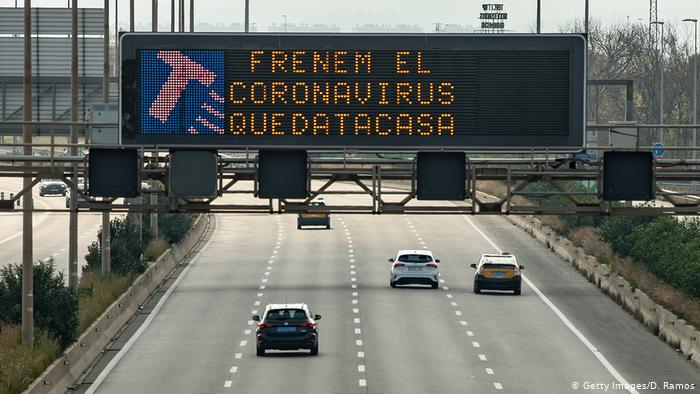
\includegraphics[width=0.8\textwidth]{52776268_303}
\caption{Awesome Image}
\label{fig:awesome_image}
\end{figure}

\section{Table}
In Table \ref{tab:my_awesome_table} we described the weather.

\begin{table}[h]
\centering
\caption{My Awesome Table}
\label{tab:my_awesome_table}
\begin{tabular}{ l l l p{2in} }
\hline
Day & Min Temp & Max Temp & Summary \\ \hline
Monday & 11C & 22C & A clear day with lots of sunshine.
However, the strong breeze will bring down the temperatures. \\ \hline
Tuesday & 9C & 19C & Cloudy with rain, across many northern regions. Clear
spells
across most of Scotland and Northern Ireland,
but rain reaching the far northwest. \\ \hline
Wednesday & 10C & 21C & Rain will still linger for the morning.
Conditions will improve by early afternoon and continue
throughout the evening. \\
\hline
\end{tabular}
\end{table}

\chapter{My Second Chapter}


\bibliographystyle{ieeetr} % IEEEtran.bst has url 
\bibliography{reference} % use .bib file auto-generated by Zotero-better-bibtex
\addcontentsline{toc}{chapter}{Bibliography}

\appendix
\chapter{Title of Appendix A}
\section{Secion Title in Appendix A}
\chapter{Title of Appendix B}


%\include{./tex/Vita_Auctoris}% Vita Auctoris (Optional)
\end{document}
